\section{Evaluation}\label{sec:evaluation}

We evaluate whether diagnostic anchor conditioning provides a more task-aligned representation for trajectory diffusion than conventional perceptual or hand-designed conditioning inputs. Our evaluation is organized around two case studies. The first considers collision avoidance, where the environment constraints are purely geometric. The second considers a richer constraint setting in which generated trajectories must satisfy both kinematic and dynamic constraints, including collision avoidance and payload-induced torque limits. Together, these studies test whether the proposed constraint-response representation remains useful when the notion of feasibility changes from simple geometric validity to a more general constraint-satisfaction problem.

\subsection{Experimental Setup}

We compare trajectory diffusion models that share the same denoising architecture and training procedure, but differ in the representation used for environment conditioning. The proposed method, denoted \textit{Anchor Traj}, conditions the model on binary constraint-response signatures induced by the selected diagnostic anchor snippets. These anchors are chosen using the entropy-based procedure described in Section~III, which greedily selects snippets whose feasibility outcomes maximally refine the current partition of training environments.

We compare against four conditioning baselines. \textit{Point Cloud} conditions the diffusion model on a point-cloud representation of the environment using a standard PointNet++ encoder. \textit{Key Config} conditions on key robot configurations produced by PRESTO. \textit{Start-Goal} provides only the planning query and does not condition on environment information. \textit{Random} assigns random vectors as environment codes, testing whether performance gains arise merely from providing distinct identifiers rather than behaviorally meaningful structure. We also report \textit{VAMP} as an oracle-like upper bound. VAMP is not intended as a directly comparable learned conditioning method; rather, it indicates the approximate performance ceiling achievable by the underlying planner or trajectory source.

All learned models are trained using three random training seeds. Error bars indicate variation across seeds. In the plots, the notation ``$k/3$'' indicates that a baseline outperformed Anchor Traj on $k$ out of three seeds for the corresponding metric.

\subsection{Metrics}

We evaluate generated trajectories using four collision-related metrics. The \textit{collision-free rate} measures the fraction of generated trajectories that satisfy collision constraints over the full trajectory. The \textit{collision steps} metric counts the number of states along a trajectory that are in collision. The \textit{collision fraction} normalizes this quantity by trajectory length, measuring the proportion of the trajectory that violates collision constraints. Finally, we compute worst-case clearance metrics over trajectories that are mostly collision-free. The \textit{mean worst-case clearance} measures the average minimum clearance along generated trajectories, while the \textit{tail worst-case clearance} reports the fifth percentile of worst-case clearance, capturing rare but severe constraint violations.

For the payload-handling case study, we additionally evaluate dynamic feasibility using torque-related metrics. In particular, we measure whether generated trajectories remain within torque limits induced by the manipulated payload and report both aggregate feasibility and worst-case torque-margin statistics. This allows us to test whether the anchor construction remains effective when feasibility depends not only on geometry, but also on dynamic constraints.

\begin{figure*}
  \centering
    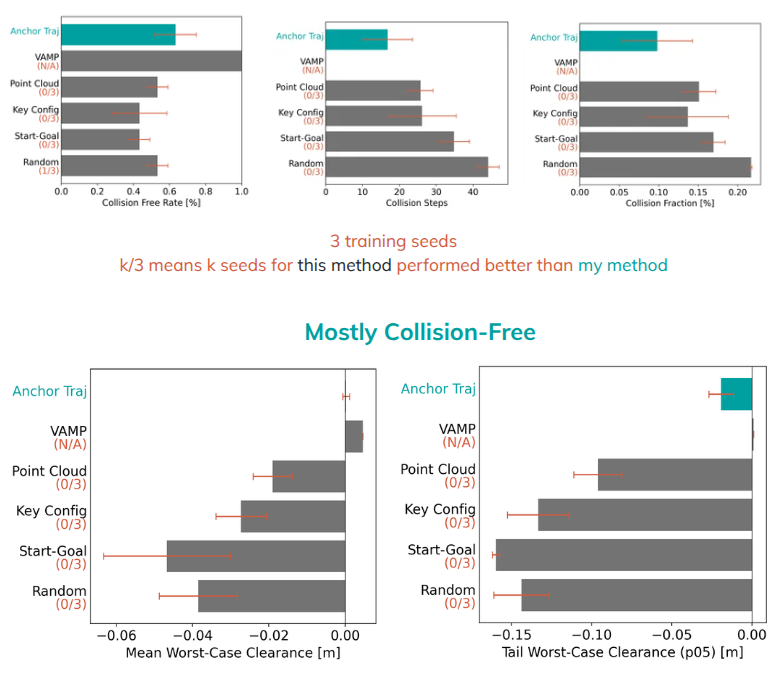
\includegraphics[width=\textwidth]{figs/eval.png}
  \caption{Collision-avoidance evaluation across three training seeds. Anchor Traj denotes the proposed diagnostic anchor conditioning method. VAMP is shown as an oracle-like upper bound rather than a learned conditioning baseline. Point Cloud uses a PointNet++ environment encoder, Key Config uses PRESTO key configurations, Start-Goal does not condition on environment information, and Random uses random environment codes. Anchor Traj achieves the strongest learned-model performance across collision-free rate, collision steps, collision fraction, and worst-case clearance metrics.}\label{fig:eval}
\end{figure*}

\subsection{Case Study 1: Collision Avoidance}

Figure~\ref{fig:collision_results} summarizes the collision-avoidance results. Anchor Traj achieves the best learned-model performance across the primary collision metrics. While VAMP provides the expected upper bound in collision-free rate, Anchor Traj produces the highest collision-free rate among learned conditioning methods. In contrast, Point Cloud and Random conditioning obtain lower success rates, while Key Config and Start-Goal perform substantially worse. This suggests that explicitly encoding constraint-response behavior provides a more useful conditioning signal than either raw geometric perception or environment-agnostic conditioning.

Anchor Traj also substantially reduces the severity of constraint violations. In terms of collision steps, Anchor Traj produces fewer colliding states than Point Cloud, Key Config, Start-Goal, and Random conditioning. The same trend is reflected in collision fraction, where Anchor Traj has the lowest fraction of trajectory states in collision among learned methods. These results indicate that the proposed representation does not merely improve binary success rate; it also shifts failed trajectories closer to feasibility by reducing the amount of time spent in violation.

The clearance results further support this trend. Among trajectories that are mostly collision-free, Anchor Traj produces the best worst-case clearance behavior of the learned methods. Both the mean worst-case clearance and the lower-tail clearance are improved relative to Point Cloud, Key Config, Start-Goal, and Random conditioning. This is especially important because worst-case clearance captures whether a generated trajectory merely avoids collision by a small margin or maintains a safer separation from obstacles throughout execution. The improved tail clearance suggests that Anchor Traj reduces rare but severe near-collision failures.

These results support the central hypothesis of this work: the most useful environment representation for trajectory diffusion is not necessarily the one that most explicitly describes scene geometry, but the one that best preserves constraint-induced behavioral distinctions. Point Cloud conditioning provides direct geometric information about obstacles, yet it must learn from data which geometric variations matter for trajectory feasibility. Anchor Traj instead exposes this information through diagnostic feasibility probes, providing the diffusion model with a compact code aligned with the obstacle-avoidance task.

\subsection{Case Study 2: Collision Avoidance with Payload-Induced Dynamic Constraints}

The second case study evaluates whether the proposed representation extends beyond geometric collision avoidance to settings involving both kinematic and dynamic constraints. In this setting, generated trajectories must remain collision-free while also satisfying payload-dependent torque constraints. This case study is designed to test the constraint-agnostic nature of the anchor selection procedure. Since anchors are selected from binary feasibility outcomes, the same procedure can be applied regardless of whether a snippet fails due to obstacle collision, kinematic infeasibility, excessive torque, or a combination of constraints.


For this experiment, we redefine the constraint oracle as a joint feasibility test:
%
\begin{equation}
    \Phi(e,\tau)=1
    \quad \Longleftrightarrow \quad
    \begin{aligned}
        &\tau \text{ satisfies collision, kinematic,}\\
        &\text{and torque constraints in } e.
    \end{aligned}
\end{equation}
%
The anchor selection procedure is then run on the resulting joint constraint-response matrix. This produces anchors that are informative with respect to the combined feasibility model rather than collision alone. As a result, the selected probes are expected to capture not only where obstacles constrain motion, but also which motions become infeasible under payload-induced torque limits.

We will evaluate this case study using the same collision metrics described above, together with torque-specific feasibility metrics. The key comparison is whether Anchor Traj continues to outperform perceptual, key-configuration, start-goal, and random conditioning when the source of infeasibility is no longer purely geometric. Strong performance in this setting would indicate that the proposed representation is not specialized to collision avoidance, but instead provides a general mechanism for constructing task-aligned conditioning inputs from arbitrary constraint models.

\subsection{Discussion}

Across the collision-avoidance case study, Anchor Traj consistently provides the strongest learned conditioning representation. The improvement over Start-Goal confirms that environment information is necessary for constrained trajectory generation. The improvement over Random shows that the benefit is not simply due to assigning distinct identifiers to environments. The improvement over Point Cloud and Key Config suggests that high-dimensional geometric or hand-designed representations may not be sufficient unless they are aligned with the downstream feasibility objective.

The oracle-like VAMP results provide useful context. VAMP indicates the performance ceiling of the underlying trajectory source and is therefore not expected to be matched exactly by learned diffusion models. However, the gap between Anchor Traj and VAMP is smaller than the corresponding gap for the other learned conditioning approaches across the collision metrics, suggesting that diagnostic anchors preserve more of the task-relevant structure needed for feasible generation.

The expected payload-handling results will further test the generality of the approach. If the same anchor selection framework improves performance when torque constraints are included, this would support the claim that diagnostic anchor selection is constraint-agnostic. In that case, the method should be understood not as a collision-specific representation, but as a general procedure for constructing behavioral environment codes from arbitrary feasibility queries.